

\subsection{量子电路}

交换两个量子比特的电路可以被表示为

\begin{figure}[htbp]
    \centering
    \begin{minipage}{12cm}
        \centering
        \Qcircuit @C=1em @R=1.2em {
        &\ctrl{1}&\targ&\ctrl{1}&\qw\\
        &\targ&\ctrl{-1}&\targ\\
        }
    \end{minipage}
\end{figure}

这是因为容易验证 \begin{align}\begin{aligned}
        \ket{a,b} & \to\ket{a,a\xor b}                              \\
                  & \to\ket{a\xor(a\xor b),a\xor b}=\ket{b,a\xor b} \\
                  & \to\ket{b,(a\xor b)\xor b}=\ket{b,a}.
    \end{aligned}\end{align}

% \subsubsection{贝尔态}

考虑在阿达码门后面跟着一个受控非门, 并对四个二维基态进行计算, 我们会得到 \begin{align}\begin{aligned}
        \ket{\beta_{0,0}}=\frac{\ket{00}+\ket{11}}{\sqrt{2}} \\
        \ket{\beta_{0,0}}=\frac{\ket{01}+\ket{10}}{\sqrt{2}} \\
        \ket{\beta_{0,0}}=\frac{\ket{00}-\ket{11}}{\sqrt{2}} \\
        \ket{\beta_{0,0}}=\frac{\ket{00}-\ket{10}}{\sqrt{2}}
    \end{aligned}\end{align}
容易发现 \begin{align}\begin{aligned}
        \ket{\beta_{x,y}}=\frac{\ket{0,y}+(-1)^x\ket{1,\overline{y}}}{\sqrt{2}}.
    \end{aligned}\end{align}
其量子电路为

\begin{figure}[H]
    \centering
    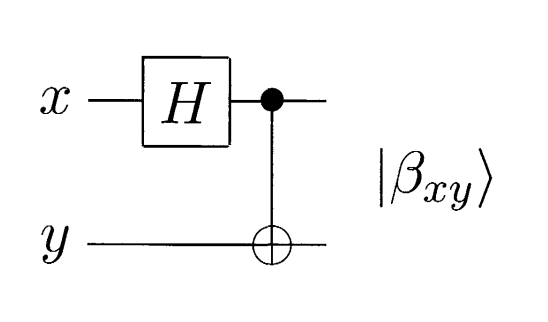
\includegraphics[width=0.4\textwidth]{pic/3.png}
\end{figure}
